\chapter{Literature Review}
\externaldocument{deep_learning_background}

This section shall discuss the currently existing datasets and models relating to visual speech recognition (VSR).
This shall be explored in both the space of two dimensional images and three dimensional scans of speaking subjects, the current successes in these fields and the current issues which are faced in progressing these areas of research forwards.

\section{Current Lip Reading Models and Datasets}

In recent years the problem of VSR, also know as lip reading, has seen huge advances due to the availability of new datasets and the use of Deep Learning models \cite{Chung2016, Chung2017, Shillingford2018}.
This section shall discuss the progresses which has already been made in this field and the datasets publicly available on which to train such models.
Current lip reading models, to the best of the author's knowledge, all make use of 2D temporal data such as videos by evaluating the frames of the video, using this information to make a prediction of the word, or words, which were spoken in the sequence.

However in reality, humans who are able to lip read also have access to three dimensional data due to our depth perception, which is not well represented in 2D video frames; thus is can be hypothesised that some information captured by 3D temporal scans of speaking subjects can also be used for speech prediction.
Unlike 2D temporal data, 3D temporal data (3D video), requires multiple cameras to record simultaneously, which in turn requires synchronisation between the cameras, increasing the complexity of the system beyond simply having multiple cameras.
The data must then be processed to produce the final product, whether this is in the form of video with depth information or more complex 3D scans \cite{Li2017}.

\subsection{Datasets}
There currently exists multiple labelled video datasets which can be used for traditional VSR; here 'traditional' refers to using 2D temporal data.
Datasets such as GRID \cite{Cooke2006}, LRW \cite{Chung2016}, LRS \cite{Chung2017} and LSVSR \cite{Shillingford2018} have been constructed by compiling the video data from various sources, each with an increasing vocabulary and dataset size.

\subsubsection{Controlled Conditions Datasets}
The GRID dataset was released in 2006 \cite{Cooke2006} and contains 34,000 samples from 34 speakers, each with 1000 sentences.
Based on previous work using the coordinate response measure (CRM) \cite{Bolia2000}, the corpus uses sentences with a fixed grammar: <command:4>, <colour:4>, <preposition:4>, <letter:25>, <number:10>, <adverb:4>, with a total vocabulary of 51 words.
Aside from the restricted vocabulary size in comparison to more recent datasets, the primary limiting factor of the GRID dataset is that all data was captured directly for the use of the dataset, and so models trained on this dataset have learnt under controlled conditions, something not found in the desired wider applications of VSR.

\subsubsection{In The Wild Datasets}
To build larger datasets more suited for deep learning models, the following are commonly built with "\textit{in the wild}" data, meaning that the original videos have not been captured with the intention of being used for this dataset, whilst the data collected for the datasets is preprocessed such that it is suited for the task.
Variations in lighting, angles, speakers and a wide vocabulary are common, this does however make the datasets more challenging to learn from, but the models are no longer as biased to controlled conditions.

LRW and LRS are both comprised of content from BBC broadcasts \cite{Chung2016, Chung2017} allowing for a far larger corpus size of 500 words for LRW and over 6000 words for LRS.
Both datasets are captured and processed with the same pipeline (Figure \ref{fig:LRW_Pipeline}) summarised as follows. 

\begin{figure}[h]
    \centering
        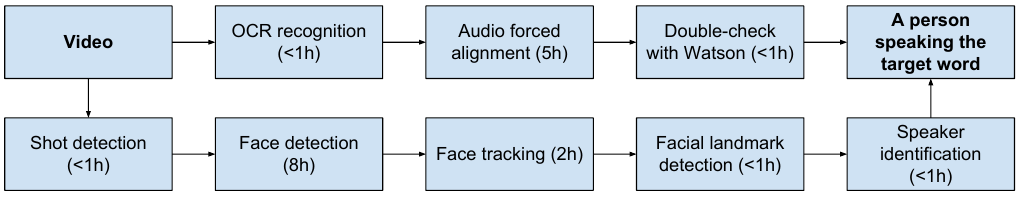
\includegraphics[width=0.95\textwidth]{figures/lit_review/lrw_pipeline.png}
    \caption{LRW Dataset Pipeline \cite{Chung2016}}\label{fig:LRW_Pipeline}
\end{figure}

Firstly, as the text transcripts are broadcast as bitmaps, optical character recognition (OCR) \cite{Buehler2009} is used to obtain the text spoken in the video, the audio and text are then aligned per frame using the HTK toolkit \cite{Woodland1995}.
The quality of these predictions are validated with the use of the commercial IBM Watson Speech to Text converter.

Secondly, face detection and tracking are used so that the frame can be cropped to feature the subject's mouth at the centre.
To achieve this, a histogram of oriented gradients based (HOG) detection algorithm \cite{King2009} is used on all video frames to detect faces, see left hand side of Figure \ref{fig:LRW_Face_Detection}.
A Kanade-Lucas-Tomasi (KLT) feature tracker is also applied to the frames, such that where HOG and KLT overlap (see centre of Figure \ref{fig:LRW_Face_Detection}), it is assumed to be tracking the face correctly.
To identify mouth position, facial landmarks are then used using an ensemble of regression trees method from \cite{Kazemi2014}, see the right of Figure \ref{fig:LRW_Face_Detection}.

\begin{figure}[h]
    \centering
        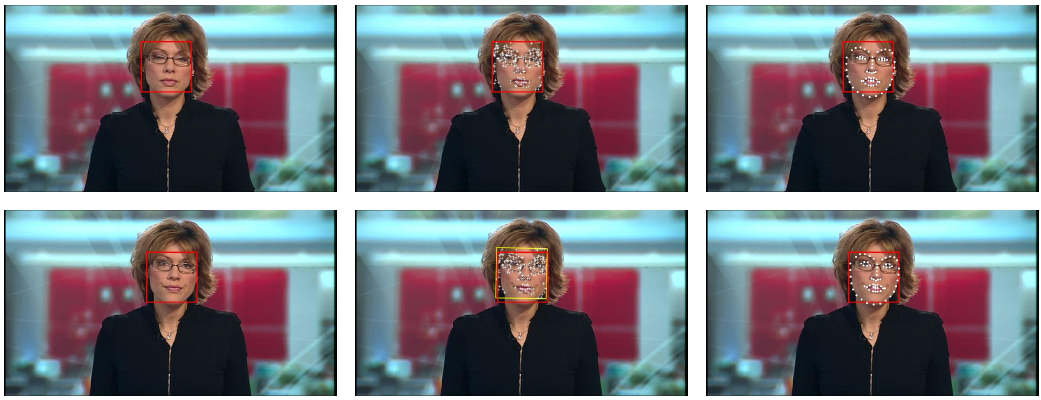
\includegraphics[width=0.99\textwidth]{figures/lit_review/lrw_face_detection.png}
    \caption{LRW Face Detection and Tracking \cite{Chung2016}}\label{fig:LRW_Face_Detection}
\end{figure}

As multiple faces can appear at any one time, it is assumed that the speaker will be the only subject with a moving mouth.
Assuming that the lip movements fall within a frequency range, the Fourier transform is applied to the openness of the mouth defined by the distance between top and bottom lip from the facial landmarks.
A support vector machine (SVM) is then trained on the frequency spectrum to classify who is speaking in each frame.
The frames are then cropped around the relevant speaker, an example of a sample from the dataset is shown in Figure \ref{fig:LRW_One_Second}.

\begin{figure}[h]
    \centering
        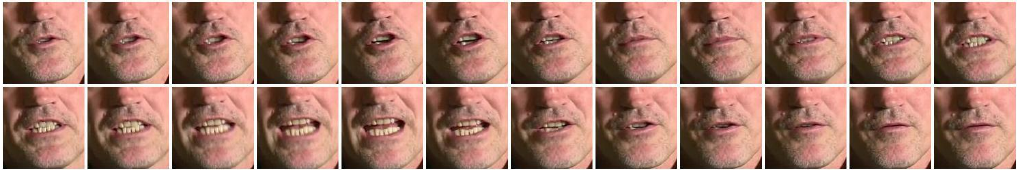
\includegraphics[width=0.99\textwidth]{figures/lit_review/lrw_one_second.png}
    \caption{LRW Dataset Sample: 24 frames of a subject saying \textit{`about'} \cite{Chung2016}}\label{fig:LRW_One_Second}
\end{figure}

LSVSR is a dataset published by DeepMind and Google which makes use of the huge amount of videos on YouTube \cite{Shillingford2018}, resulting in a total length of 3886 hours of training data.
Unlike LRW or LRS, LSVSR aligns phonemes to frames, as opposed to words or characters.
The pre-processing steps are similar as in LRW and LRS, although the alignment is performed with the algorithm laid out in previous work by DeepMind \cite{Liao2013}.

\subsubsection{3D Datasets} \label{3D Datasets}
To the best of the author's knowledge, there are currently only two datasets with 3D temporal data which could be appropriate for training lip reading models, neither of which have been captured with the intention of being used for VSR.

The first of which is LRW-3D \cite{Tzirakis2019} which has been captured from four subjects, two native English speakers and two non-native to increase variability in the dataset.
The subjects have been captured speaking the corpus used in the LRW dataset \cite{Chung2016}, a vocabulary of 500 words.
The resulting dataset comprises of 660 seconds of 3D meshes and audio per subject.
The dataset is not comprised of full sentences but would be appropriate for word-level lip reading, however a total duration of 660 seconds is likely to be too short for a deep learning model to train effectively.
The dataset had also not been officially published at the time of this report.

The second is the VOCASET \cite{Cudeiro2019}, an unlabelled dataset captured from 6 male and 6 female subjects.
Each subject was recorded speaking 40 sequences, each ranging from 3 to 5 seconds, resulting in a total time of 30 minutes.
The recorded 3D meshes are registered to the FLAME model \cite{Li2017}, a statistical 3D facial mesh with around 5000 vertices, an example sample from the dataset can be seen in Figure \ref{fig:VOCASET_example}.
Unlike the LRW-3D dataset, the sequences are grammatically correct sentences, chosen to maximise phonetic diversity.
This makes the VOCASET appropriate for creating a model for sentence-level lip reading.
Similarly to LRW-3D, 30 minutes of training data is likely to be a limiting factor when training a deep learning model.

\begin{figure}[h]
    \centering
    \begin{subfigure}[b]{0.19\textwidth}
        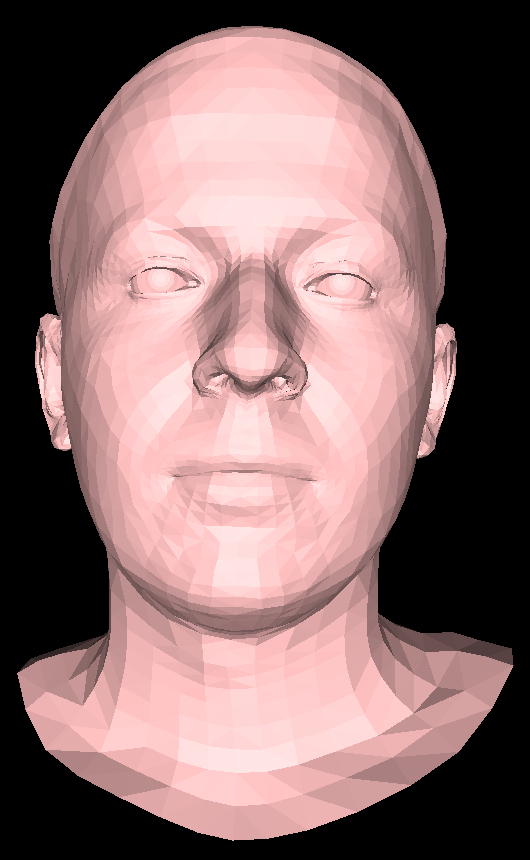
\includegraphics[width=\textwidth]{figures/voca_exp/vocaset_exp1.png}
    \end{subfigure}
    \begin{subfigure}[b]{0.19\textwidth}
        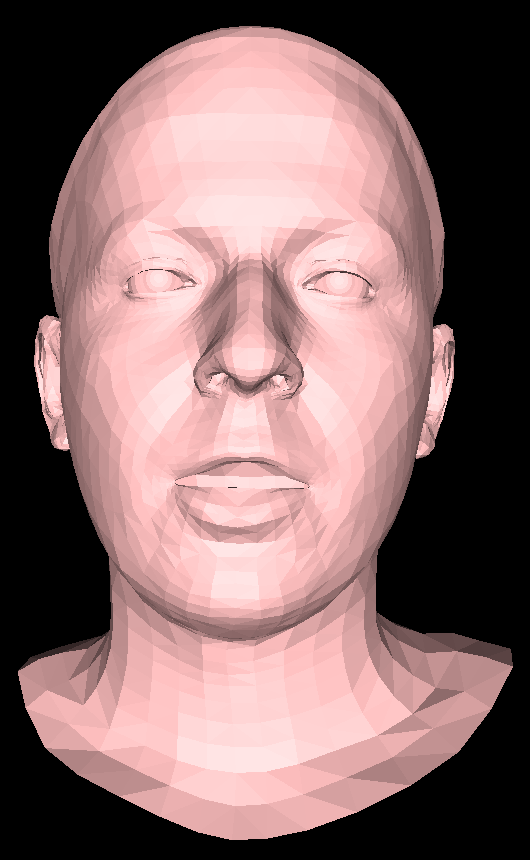
\includegraphics[width=\textwidth]{figures/voca_exp/vocaset_exp2.png}
    \end{subfigure}
    \begin{subfigure}[b]{0.19\textwidth}
        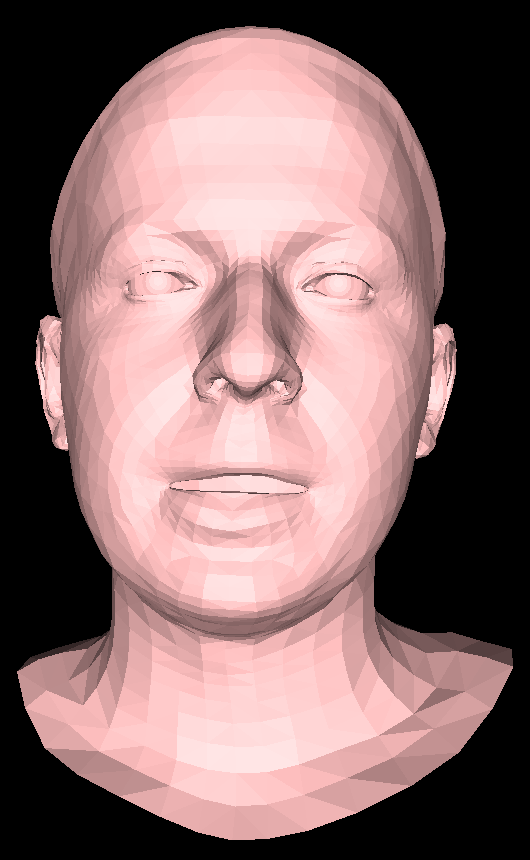
\includegraphics[width=\textwidth]{figures/voca_exp/vocaset_exp3.png}
    \end{subfigure}
    \begin{subfigure}[b]{0.19\textwidth}
        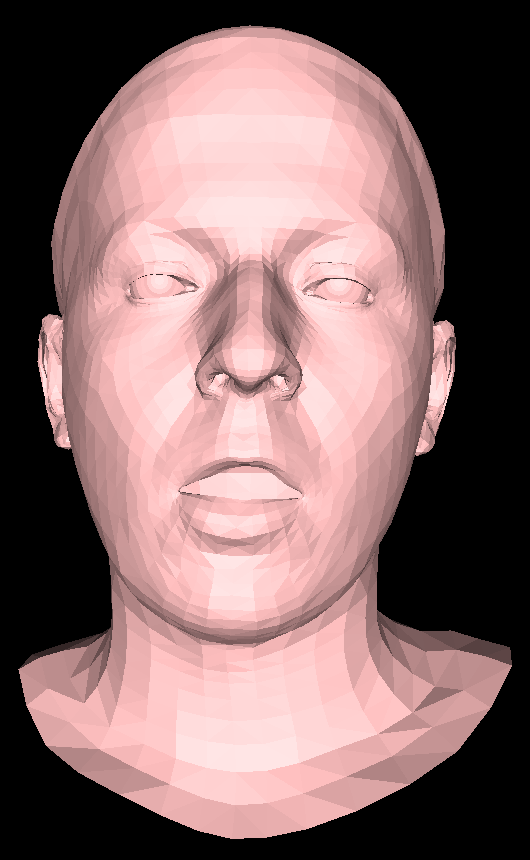
\includegraphics[width=\textwidth]{figures/voca_exp/vocaset_exp4.png}
    \end{subfigure}
    \begin{subfigure}[b]{0.19\textwidth}
        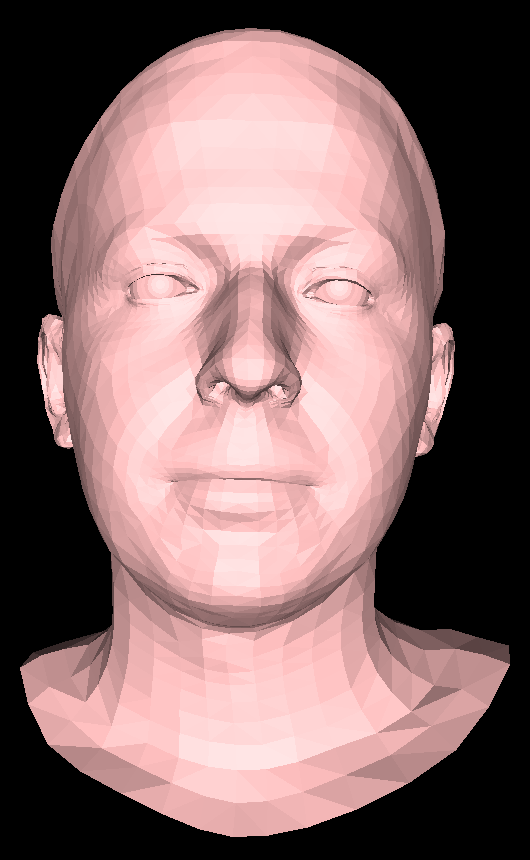
\includegraphics[width=\textwidth]{figures/voca_exp/vocaset_exp5.png}
    \end{subfigure}
    \caption{VOCASET Example Frames \cite{Cudeiro2019}}\label{fig:VOCASET_example}
\end{figure}

It should be noted that neither of these datasets were captured for the purpose of lip reading, but for synthesising realistic statistical facial models driven from an audio input, and thus there are no transcriptions for VOCASET.
The transcriptions could be obtained with an Audio Speech Recognition (ASR) method such as DeepSpeech \cite{Hannun2014} and then alignment would have to be performed to the datasets before using the data to train lip reading models.

\subsection{Lip Reading Models} \label{sec:lip_reading_models}
In \cite{Chung2016} Chung et al. used a multiple towers convolutional model based on the VGG-M architecture for multi-label classification to classify a video clip to one of the five hundred labels in the LRW dataset.
The model architecture (Figure \ref{fig:LRW_Multiple_Towers}) first processes each frame separately with a shared convolutional layer to extract features from each frame.
These features are down-sampled with a pooling layer before being concatenated into a single high channel feature map.
A one dimensional convolutional layer then reduces the channels of this feature map before being processed by subsequent convolutional and pooling layers.
The final layer of the model is passed through a softmax activation function to predict one of the 500 word labels, see section \ref{softmax}.

\begin{figure}[h]
    \centering
        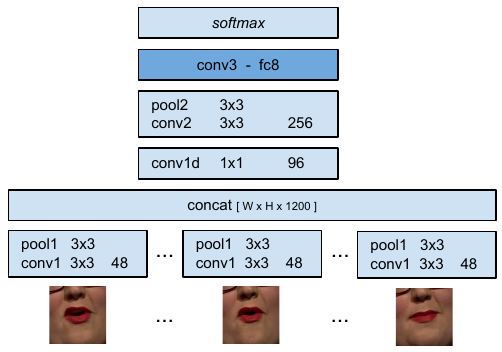
\includegraphics[width=0.7\textwidth]{figures/lit_review/lrw_multiple_towers.png}
    \caption{LRW Multiple Towers Convolutional Neural Network Model \cite{Chung2016}}\label{fig:LRW_Multiple_Towers}
\end{figure}

Chung et al. suggest that the multiple towers model is effective due to the delay in time domain operations until after the first convolutional layer which allows for tolerance to registration errors in the dataset.

As well as measuring the performance of the model on total prediction accuracy, \cite{Chung2016} also uses character-level edit distance, measured as the minimum number of characters required to be changed in the predicted label to obtain the ground truth.

The LipNet model \cite{Assael2016} was the first model produced to be able to predict end-to-end sentence-level lip reading of varied length, while previous work predicted on a word level.
The model used spatiotemporal convolutions to process multiple frames of video at once followed by a recurrent layer using Gated Recurrent Units (GRUs) \cite{Cho2014} and made character level predictions.
The model used the GRID dataset \cite{Cooke2006} due to it being the largest sentence level dataset at the time, on which LipNet achieved the state of the art performance.

As the LRW dataset could not be used to train a model such as LipNet for sentence-level lip reading, but the GRID dataset had limitations in the number of subjects and vocabulary, Chung et al. created the LRS dataset \cite{Chung2017}.
The model presented in \cite{Chung2017} was trained on both audio and video and made capable of taking either or both as the model inputs.
To prevent the model from being dependent on a single input source, the inputs are systematically distorted or removed.
The video input is passed through convolutional layers, followed by LSTM (Long Short-Term Memory) layers \cite{Cheng2016}, while the audio is converted to Mel-frequency cepstral coefficients (MFCC), then input to LSTM layers.
The two are combined with the attention mechanism and further LSTM layers and an output fully connected layer with softmax activation for character level predictions.
The model also makes use of curriculum learning by initially training the model on short sequences of single words, before increasing the length of training sequences during training.
It is stated by \cite{Chung2017} that this accelerates training and reduces overfitting.

In 2018 DeepMind published their V2P (Video to Phonemes) model \cite{Shillingford2018} along with the LSVSR dataset built from content from YouTube. 
LSVSR greatly surpassed all previous datasets in size and variation, containing 3886 hours of training data.
The model follows a similar architecture to LipNet \cite{Assael2016} using spatiotemporal convolutional layers followed by recurrent layers, however it used an increased number of convolutional layers and used LSTM layers in place of GRUs.
It should be commented that the size of the model and dataset dictated the use of 64 GPUs for training to allow a batch size of 128.
Unlike previous models, the V2P model predicts phonemes as opposed to characters, these phonemes are then processed by a language model for word prediction as with previous models.

To the best of the author's knowledge, there do not currently exist any papers which have explored the use of 3D temporal datasets for use with lip reading models. 
This is likely due to the shortage of 3D temporal data due to the difficulties in obtaining such data, on which such models could be trained on.

\section{Data Generation}
In order to construct a deep learning lip reading model capable of being trained on 3D temporal data, appropriate datasets must first be established.
Existing datasets \cite{Tzirakis2019, Cudeiro2019} discussed in section \ref{3D Datasets} have been captured directly with the use of multi-camera capture rigs under controlled conditions.
The total duration of both of these datasets is very short in comparison to the video datasets such as LRW, LRS and LSVSR, which is a limiting factor to the models which could be trained using them.

As the models also use different mesh models to represent the data that has been captured this also prevents the two datasets being joined directly.
Unlike 2D video data, there currently lacks a large body of 3D video data which is publicly available, limiting the construction of 3D datasets to directly capturing more 3D scans with multi-camera capture rigs, similar to those used in \cite{Tzirakis2019, Cudeiro2019} and generating synthetic training data.

\subsection{Audio Driven Data Generation}
Karras et al. proposed a method for generating 3D facial animation from audio with the use of a CNN architecture \cite{Karras2017a}, see Figure \ref{fig:Karras_Model}.
The model is actor specific, but restricting this allowed for the model to be trained on just 3-5 minutes of data per actor.
Firstly, a fixed function auto-correlation layer is used to extract a time-varying sequence of speech features from the audio input, named the formant analysis layer.
Then five convolutional layers are used to extract short-term animation features from the formant analysis network layer.
This is then followed by five convolutional layers, with each input concatenated with a learned emotional state representation.
Finally two linear layers are used to drive vertex positions from a starting mesh of the given actor.

\begin{figure}[h]
    \centering
        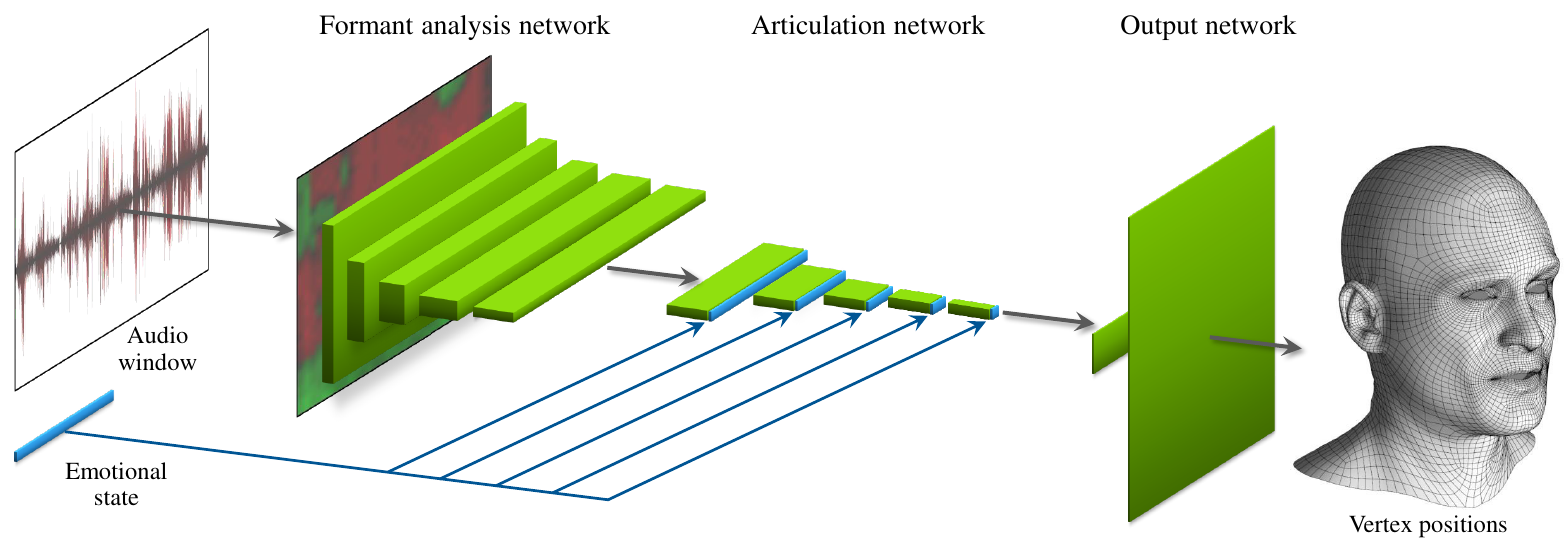
\includegraphics[width=0.9\textwidth]{figures/lit_review/karras_model.png}
    \caption{Audio Driven Facial Animation Model Proposed by Karras et al. \cite{Karras2017a}}\label{fig:Karras_Model}
\end{figure}

However, as the model by Karras et al. is not independent of the actor it cannot generalise to new subjects.
Tzirakis et al. propose a model which is independent of speaker and capture rig \cite{Tzirakis2019}.
As discussed in section \ref{3D Datasets}, a dataset was constructed of 3D speaking faces using the LRW dataset \cite{Chung2016} for the corpus.
This allowed Tzirakis et al. to create a model which can synthesise facial motion from audio from the LRW dataset.
The model used is similar to that used in \cite{Karras2017a}, firstly extracting short term temporal features from the input audio with a convolutional network followed by another convolutional network to analyse the extracted features.
Unlike the model used in \cite{Karras2017a}, the model used in \cite{Tzirakis2019} is trained to drive learnt blendshapes as opposed to vertex positions.
This reduces the number of output parameters of the model substantially in comparison to that used by Karras et al. whilst reducing the potential expressions possible to be produced by the model.

\begin{figure}[h]
    \centering
        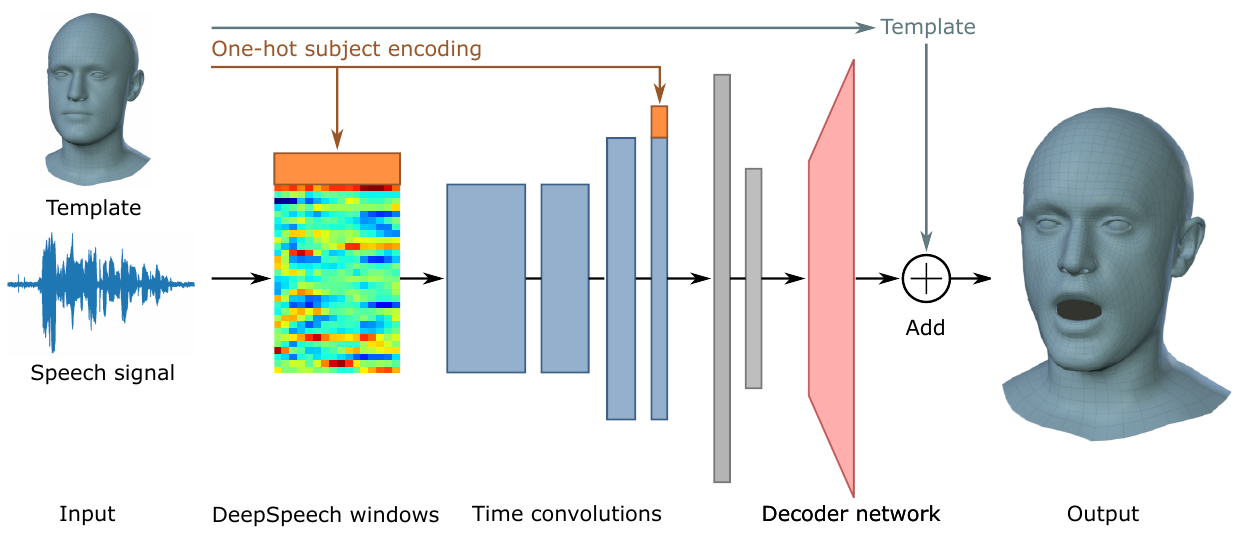
\includegraphics[width=0.9\textwidth]{figures/lit_review/voca_model.png}
    \caption{The VOCA Model \cite{Cudeiro2019}}\label{fig:VOCA_model}
\end{figure}

Similar to \cite{Tzirakis2019}, the VOCA model \cite{Cudeiro2019} synthesises video sequences of 3D models speaking given an audio input, see Figure \ref{fig:VOCA_model}.
The VOCASET dataset discussed in section \ref{3D Datasets}, was captured with the intention of training this model to be independent of the speaker, hence a large range of speaker's are used within the dataset.
The model is comprised of three sections: audio feature extraction, a feature encoder and a decoder to drive a template facial mesh from the FLAME model \cite{Li2017}.
The audio feature extraction makes use of the pre-trained Mozilla implementation of the DeepSpeech model, based on the paper by Hannun et al. \cite{Hannun2014}.
The DeepSpeech model takes audio as an input and returns the unnormalised log-probabilities for an alphabet of the 26 standard characters, a space, apostrophe and blank character for time slices in the audio input.
The encoder is a convolutional network which is conditioned on the speakers identity, such that the latent space of speaker styles can later be explored on new audio inputs.
Finally, the decoder is made up of a fully connected layer with a linear activation function used to output the displacements of the 5023 vertices in the template face.
However, as the model is conditioned with the label of which speaker the input data is from, the model does not truly learn to generalise to multiple speakers, but learns each speaker separately, thus not being independent of the speaker.

\subsection{Generative Adversarial Networks}

A recent development in generating synthetic data samples is the use of generative adversarial networks (GANs) \cite{Goodfellow2014}.
The concept behind GANs is to have two machine learning models; a generator and a discriminator.
The task of the generator is to produce samples from an unknown high order probability distribution which correctly resemble samples from the distribution defined by training data.
The generator achieves this by transforming a random sample from a known probability distribution, such as a Gaussian distribution as used in \cite{Goodfellow2014}, to a sample from the unknown distribution.
This is achieved by finding the function which maps between the two distributions.
The discriminator however, attempts to correctly learn to discriminate between the real and the generated samples.

The original loss function (\ref{eq:gans_loss}) proposed by Ian Goodfellow \cite{Goodfellow2014} forms a min-max game, where the loss of the generator is attempting to be minimised by having the discriminator label all the generated samples as real, while the loss of the discriminator is maximised by correctly classifying real and fake samples.
Here $\bm{x}$ represents the real data samples from an unknown probability distribution $p_{data}$ and $\bm{z}$ represents a random noise sample from a known distribution.
The two networks are trained in an alternating fashion until the discriminator achieves an accuracy of 50\% on real and generated samples, effectively making binary guesses between the two.

\begin{equation} \label{eq:gans_loss}
    \min_{G} \max_{D} V(G, D) = \E{\bm{x} \sim p_{data}(\bm{x})} [\log D(\bm{x})]
                              + \E{\bm{z} \sim p_{z}(\bm{z})} [\log (1 - D(G(\bm{z})))]
\end{equation}
\quad

GANs however, are difficult to train for two main reasons.
Firstly, the equation (\ref{eq:gans_loss}) is challenging as it provides small gradients while generated samples are poor as discussed in \cite{Goodfellow2014}.
Progress in developing new loss functions is discussed in section \ref{sec:Stability_to_GANs}
Secondly, early networks must also be balanced with a similar model capacity to prevent one from getting too much better than the other, preventing the other from improving.
Various architectural changes have improved this issue \cite{Radford2016, Zhang2018}, although it seems to be closely tied to the loss function being used \cite{Gulrajani2017}.

\subsubsection{Stability Improvements of GANs} \label{sec:Stability_to_GANs}
There have been a large number of papers presenting new techniques with differing levels of success and training stability, a small handful of key papers which provide large advances in the generative adversarial training model shall be discussed here.
A primary research focus around GANs has been in finding new loss functions on which to train the model to improve stability and performance.
The original loss function proposed in the original paper \cite{Goodfellow2014} identifies an issue with equation (\ref{eq:gans_loss}) in that the gradient back propagated to the generator when the generated samples are poor, is very low as shown in figure \ref{fig:Goodfellow_plot}.

\begin{figure}[h]
    \centering
        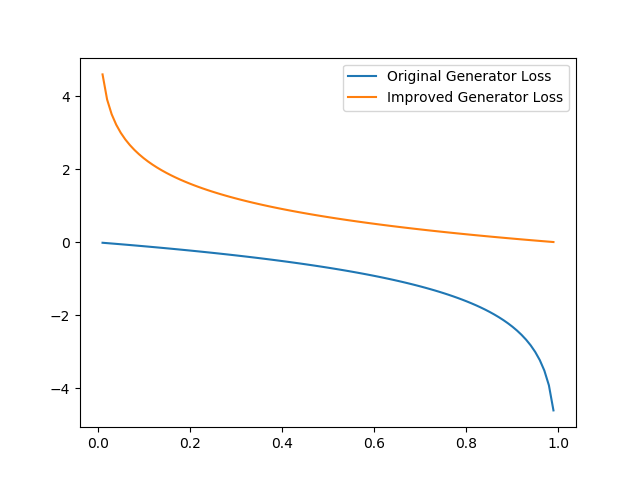
\includegraphics[width=0.8\textwidth]{figures/dl/goodfellow_gen_losses.png}
    \caption{Goodfellow's Generator Loss Plots \cite{Goodfellow2014}}\label{fig:Goodfellow_plot}
\end{figure}
\quad

This in turn makes it very challenging to improve the performance of the generator.
The suggested improvement made in \cite{Goodfellow2014} is rather than to maximise the number of generated samples which the discriminator incorrectly classifies, instead to minimise the number of generator samples the discriminator correctly classifies, as described in equation (\ref{eq:gans_loss2}).
Figure \ref{fig:Goodfellow_plot} shows how this results in the gradient propagated back to the generator is far larger when the generated samples are poor.

\begin{equation} \label{eq:gans_loss2}
    \min_{G} \max_{D} V(G, D) = \E{\bm{x} \sim p_{data}(\bm{x})} [\log D(\bm{x})]
                              - \E{\bm{z} \sim p_{z}(\bm{z})} [\log (D(G(\bm{z})))]
\end{equation}
\quad

Further stability improvements were proposed in \cite{Radford2016} which allowed deep convolutional generative adversarial networks (DCGANs) to be successfully trained for the first time.
Radford et al. proposed three main contributions.
\begin{itemize}
    \item Replace deterministic pooling layers with strided convolutions in both the generator and discriminator networks, allowing the networks to learn their own spatial upsampling and downsampling.
    \item Remove all fully connected layers used on top of convolutional layers, resulting in a fully convolutional model.
    \item Apply batch normalisation \cite{Ioffe2015} before the input of each layer.
    This normalises the input to each model layer to zero mean and unit variance.
    Batch normalisation assists with training difficulties due to poor weight initialisation and allows gradients to flow through deeper networks more easily.
\end{itemize}
Radford et al. state these to be critical improvements to allow generator networks to begin learning by preventing all samples from collapsing to a single point. 

In an attempt to stabilize the training of GAN models, the Wasserstein or 'Earth Mover Distance' loss function was proposed by Arjovsky et al. \cite{Arjovsky2017} shown in equation (\ref{eq:wgan}) where $\mathcal{D}$ is a set of 1-Lipschtiz functions.

\begin{equation} \label{eq:wgan}
    \min_{G} \max_{D \in \mathcal{D}} W(\Pd{r}, \Pd{g}) =
            \E{\bm{x} \sim \Pd{r}} [D(\bm{x})]
            -\E{\bm{\hat{x}} \sim \Pd{g}} [D(\hat{\bm{x}})]
\end{equation}
\quad

The Wasserstein GAN (WGAN) model uses a critic as opposed to a discriminator, this is due to the fact that the discriminator is no longer a binary classifier, but being used to critique the real and generated samples. 
As the Wasserstein function is continuous and differentiable, the critic can be trained until optimality, and \cite{Arjovsky2017} argues that it should be.
As the critic is trained to optimality it does not saturate, but converges to a linear function.
This provides the generator with a gradient which is more reliable, resulting in the generator learning consistently.
The Wasserstein loss function has been shown to greatly improve training stability by providing consistent gradients throughout training and no longer requires that the two networks have a balanced model capacity.

In order to use the Wasserstein distance as the loss for WGAN, the Lipschtiz condition must be enforced.
In the WGAN the model weights are clipped to enforce this constraint \cite{Arjovsky2017}, however this is stated to be a non-ideal method of achieving the Lipschtiz constraint and calls for future work to investigate more effective methods.
The use of gradient penalty is proposed in \cite{Gulrajani2017} in order to satisfy this condition more elegantly by minimising the Critic's loss function as described in equation (\ref{eq:wgan_gp}).

\begin{equation} \label{eq:wgan_gp}
    \textit{L}
        = \E{\bm{\tilde{x}} \sim \Pd{g}} [D(\tilde{{\bm{x}}})]
        - \E{\bm{x} \sim \Pd{r}} [D(\bm{x})]
        + \lambda \E{\bm{\hat{x}} \sim \Pd{\bm{\hat{x}}}} 
            [(\| \nabla_{\bm{\hat{x}}} D(\bm{\hat{x}}) \| - 1)^2]
\end{equation}
\quad

Using the Wasserstein loss function with gradient penalty enforces the Lipschtiz condition and allows highly complex architectures to be trained successfully, including those with residual units \cite{Gulrajani2017}.

\subsubsection{Architectural Developments}
Mirza et al. showed that GANs could be trained with conditional inputs to the generator network in addition to the noise component \cite{Mirza2014}.
This has facilitated other uses of GANs such as image to image translation for style transfer \cite{Zhu2017}.
Vougioukas et al. used a temporal model to generate a sequence of video frames given an image of a subject and an audio sequence of spoken text to synthesise the subject speaking \cite{Vougioukas2018}.
The model uses two discriminators, one to determine if individual frames are realistic images of the subject's face and a second which evaluates the sequence of video frames to determine if it is realistic.
The model uses temporal components to examine if the frames of video are consistent in time, preventing sudden jumps in facial position.

Other novel architectures include the progressively growing GAN model \cite{Karras2017b} which is able to generate highly realistic images of faces to a high resolution.
This is achieved by initially training a shallow model to produce 4x4 pixel images before increasing the depth of the network and training further at a higher resolution.
By forcing the model to firstly produce and examine low resolution images, the model has to be able to synthesise simple low level features effectively, such as facial shape which is common to all samples.
Once the model can produce these features a higher resolution is used, allowing it to learn more complex features, such as hair and eyes.

The attention mechanism \cite{Vaswani2017} has been shown to be useful when applied to image data \cite{Xu2015} in order to capture relationships between spatially distant points.
As such points are further apart in the image, previously deeper convolutional models were required to allow a large enough receptive field to capture information on these two points.
Zhang et al. point out that this is a common issue with DCGANs \cite{Radford2016}, where generated samples fail to produce structural patterns, while they do exceedingly well at local textural patterns.
This is often seen in generated images of animals with realistic fur, but oddly shaped or an incorrect number of limbs.
The attention mechanism is applied to GANs \cite{Zhang2018} to allow for long range dependencies in the image to be modelled by convolutional models more effectively.

To the best of the author's knowledge, there currently exists no generative adversarial networks which aim to generate 3D facial models with speech audio as a conditional input.

\section{Summary of Related Literature}
Visual speech recognition has seen large improvements in recent years, progressing from word level prediction on a relatively small vocabulary set \cite{Chung2016}, to variable length sequences predicting a sequence at a sentence level with the use of recurrent networks making character level predictions to construct the completed sentence \cite{Shillingford2018}.
These advances have come in tandem with the increase in the size and variation of the datasets on which to train such models.
While there currently exist no datasets made up of 3D temporal data which have been constructed with the intention of lip reading, there has been progress in the area of 3D model generation from an audio input.
A proposed solution to this problem would be to generate synthetic 3D temporal data by using a generative model, allowing a VSR classifier to be trained on the resulting dataset.
The model by Karras et al. is currently not publicly available due to being researched in collaboration with Nvidia.
The VOCA model however, is publicly available, although how independent the model truly is of the speakers it was trained on is unclear.
The VOCA model also has additional dependencies on the DeepSpeech model and thus is not trained fully end-to-end, potentially losing some information which might be of use for driving facial animation.
A currently unexplored area of research is the use of GANs driven by audio to generate 3D temporal data of speaking subjects.
